%!TEX root = thesis.tex

\chapter{The Building Blocks of Crowd Behavior during Egress}
\label{chapter:IBEVAC}

In the previous chapter, the salient features of the behavior of a crowd engaging in egress were introduced. It is understood that people don't immediately exit a building on hearing a fire alarm or seeing smoke. The occupant gets only an inkling about the danger that is possible. In both these cases there is not enough information for him to get scared and make the decision to egress. If the cues are interesting enough, he then embarks on investigating to gather more information. On realizing that the situation requires some action, he forms a plan to evacuate either alone or, if possible, with his primary group members. In forming this plan of evacuation, unless he is trained for egress or very familiar with the environment, it is unlikely that he will have knowledge of all exits. As a result, he is most likely to just move to the nearest \emph{known} exit. An overview of this process of human evacuation is illustrated in Fig.~\ref{fig:EvacuationProcess}.
% Whatever action they are undertaking, they preserve social norms as far as possible by not shoving or pushing other people~\cite{Cocking:2005uc,Drury:2009ga,Torres:2010tj}.
\begin{figure}[!htb]
\centering
\includegraphics[height=4in]{fig-ProcessOfEvacuation}
\caption[The Process of Evacuation]{The Process of Evacuation: This state diagram shows the different phases of behavior of a person engaging in egress and the triggers that cause phase changes}
\label{fig:EvacuationProcess}
\end{figure}
%  Change this figure!

% The previous chapter also introduced various approaches that have been used for computationally modeling egress behavior. Section~\ref{LiteratureReview:DetailedModels} presented some of the models that simulated human behavior most accurately and almost all of these used an Agent Based Modelling approach. Agent Based Modelling is the preferred approach for modeling complex behavior~\cite{Epstein:1999vn} because the bottom up approach makes it easier to view and break down problems into more manageable entities. What exactly are agents? Woolridge~\cite{IntelligentAgentsWoolridge} defines agents as a computer system that is situated in some environment, and that is capable of autonomous action in this environment in order to meet its design objectives. He further defines Intelligent agents as those agents that are capable of flexible autonomous action through reactivity, pro-activity and social ability. In order to create an agent based model, the software architecture used for modeling this decision making ability needs to be detailed. This is called the Agent Architecture. Specifying an architecture would provide a structure that can be used to break down the complicated process of decision making. There are several frameworks like the Belief-Desire-Intention (BDI) framework~\cite{BDI} and the Recognition Primed Decision (RPD) that provide a structure on which agent based architectures can be developed. However, simply saying that a BDI or an RPD architecture is used does not help in creating or understanding the agents. They simply provide the guiding principle of the model.

% Despite the usefulness of an agent architecture, for most models the agent architecture used is not provided. Figure~\ref{fig:ExistingAgentArchitectures} shows the architectures of some agent based models of egress that outline the architecture used. Figure~\ref{fig:MASSEgressAgentArchitecture} and Figure~\ref{fig:LinboAgentArchitecture} describe the simulation architecture more than the agent architecture. The behavior model used in MASSEgress is only defined as pseudo-code and the agent architecture itself is not explicitly defined. Luo et al.~\cite{Luo:2008gj} also take a similar approach of describing their model in text with the architecture simply showing the behavior as being a result of the interaction between situational awareness, agent attributes and behavior execution. Shendakar et al.~\cite{BDIModel} do provide the actual BDI based agent architecture that they use for their simulation( Figure~\ref{fig:BDIModelArchitecture}). However, by defining all memory of an agent simply as \emph{beliefs} and actions as \emph{actuators} the architecture oversimplifies complicated problems that need to be analyzed in more detail. This limits the architecture's general usefulness in studying computational modeling of egress beyond the specific way in which it is used.

% In this chapter, we introduce the IBEVAC Agent Architecture for modeling behavior of evacuees in an agent based simulation. The chief motivation of this model is to identify and modularize the key building blocks of the behavior of an agent approximating an evacuee.  It is generally recognized that information plays an important part in solving problems~\cite{Simon:1970th} and other daily decisions. Moreover, information perception and processing is the common theme running through the different steps of the egress procedure outlined above. Using this underlying theme of an evacuee being primarily an information processing entity, an agent based framework called \emph{Information Based EVACuation} (IBEVAC) model is introduced in this chapter.


Section~\ref{IBEVAC:EgressProgress} explores how this evacuation process can be produced as a result of the interaction of a small set of subprocesses. Section~\ref{bladerasdf} gives an overview of how the following chapters identify and solve key shortcomings in existing models of these aspects.

% introduces some existing architectures and the need for a new agent architecture. This division is used as the basis for the IBEVAC agent architecture that is described in Sect.~\ref{IBEVAC:AgentArchitecture}.


% \begin{figure}[!t]
%   \centering
%    \subfloat[BDI Based model~\cite{BDIModel}]{\label{fig:BDIModelArchitecture}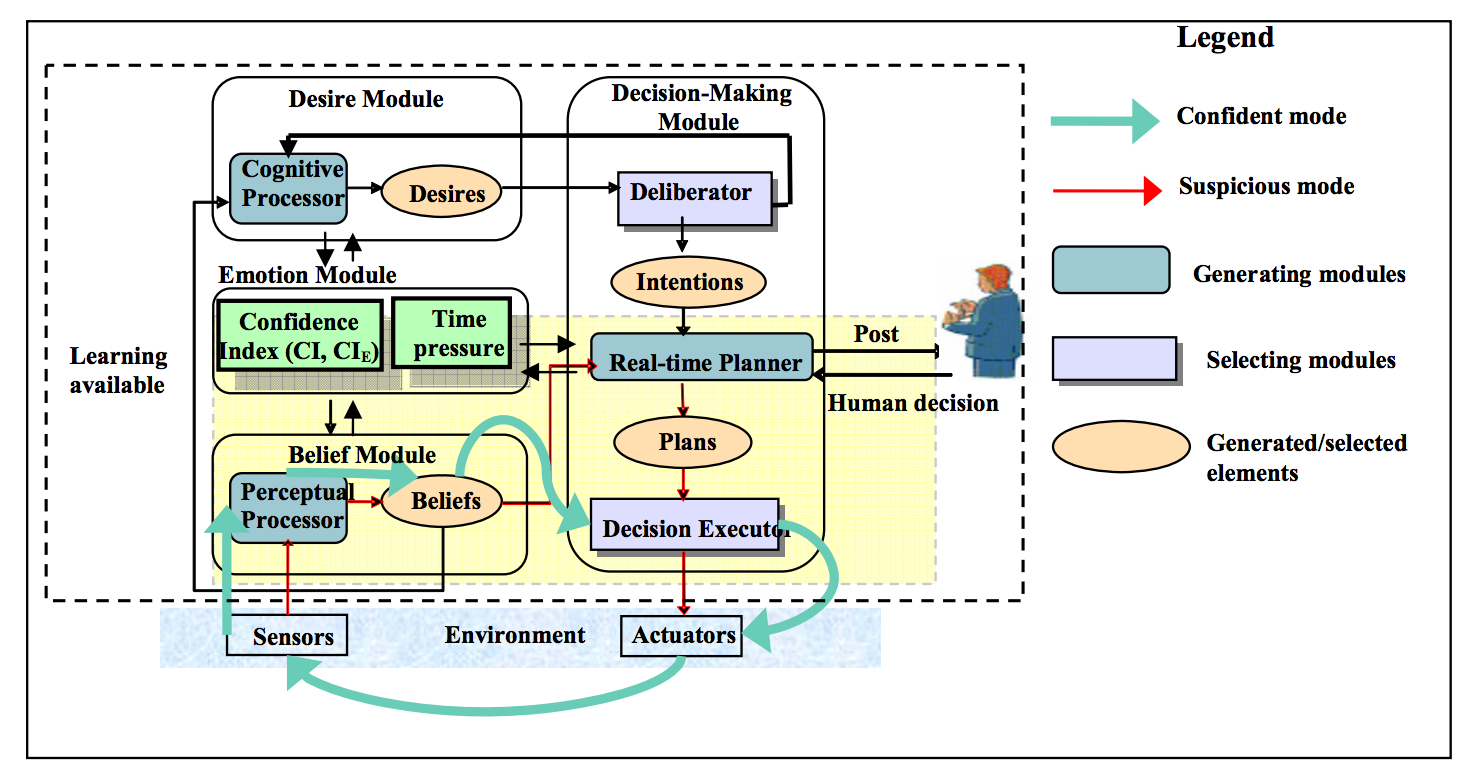
\includegraphics[height=7cm]{BDIModel}}
%   \\
%     \subfloat[MASSEgress model~\cite{Pan:2006vp}]{\label{fig:MASSEgressAgentArchitecture}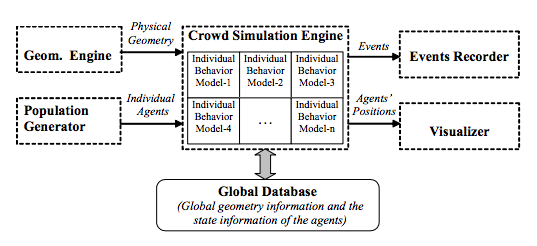
\includegraphics[height=7cm]{Massegress-Architecture}}
%   \\
%   \subfloat[Model proposed by Luo et al.~\cite{Luo:2008gj}]{\label{fig:LinboAgentArchitecture}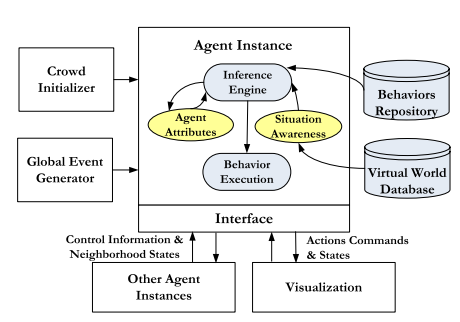
\includegraphics[height=7cm]{LinboModel}}
%   \caption{Existing Agent Architectures}
%   \label{fig:ExistingAgentArchitectures}
% \end{figure}




% section existing_agent_architectures (end)

\section{The Egress Process}
\label{IBEVAC:EgressProgress}

The evacuation process outlined earlier in this chapter and discussed in more detail in the last chapter can be simulated with the help of four major building blocks: perception, event identification, knowledge and navigation. This section explains how this is possible by defining each of these building blocks and their significance in the evacuation process.

\subsection{Perception}
\label{IBEVAC:IBP}
	Perception refers to the process by which an environment is observed by a person. For an agent, this implies that it should extract features from the environment. These features are called percepts~\cite{Russel:1995vi}. At the simplest level, percepts provide the agent information about the location and motion of other dynamic agents and thus allow it to avoid collisions and move naturally. In some cases, something out of the ordinary like a ringing fire alarm or smoke or even people running away from a location, might be perceived. If these special percepts, known as \emph{cues}, are intriguing enough, then the occupant will set about investigating the environment in search of more cues that would help make a decision on a plan of action. The percepts can also be in the form of messages sent to the evacuee from other evacuees. Each percept~(whether it is a cue or not) gives the evacuee certain information about the environment. The perception process is the main interface of the agent with the environment through which it gets all the information needed to act.
    % This idea of looking at perception as a process of gathering information is referred to, in this thesis, as \emph{information based perception}.

\subsection{Event identification} % Funky name needed
\label{IBEVAC:EventIdentification}
	On perceiving \emph{enough} cues from the environment, an evacuee stops whatever task he's doing and initiates a process of investigation. Once enough evidence is gathered to convince the evacuee of danger, evacuation starts; if there is not enough information then the evacuee will probably go back to doing whatever he was doing earlier. Thus identification of events is a key component of the evacuation process and it's essential for modeling the pre-evacuation behavior discussed in the previous chapter.

    How do the evacuees decide that the information gathered is \emph{sufficient}? A person's intrinsic characteristics like age, gender and mental state determine how much information is considered enough i.e.\ the threshold. Each person keeps a track of all the cues that are perceived and when the amount of information crosses the threshold, the evidence is acted upon. In the first phase mentioned above, this action would be to start investigation and in the second phase it would be the starting of the process of evacuation. In this thesis, this whole process by which the evacuee perceives, analyses and aggregates cues and identifies an event is called \emph{event identification}. Event identification is the process by which the evacuee decides to proceed to the next phase of evacuation.

\subsection{Evacuation planning}
\label{IBEVAC:Knowledge}
	On recognizing that there is a fire to escape from, the evacuee tries to find his primary group members and then moves towards the closest known exit. Each evacuee holds his own personal version of the map of the environment which is used for evacuation and movement in general. This personal map is not necessarily accurate. Also, more importantly, in a lot of cases, it is not complete. In a scenario where all known exists are blocked or if the evacuee does not know any exit, he/she is likely to engage in some sort of exploration behavior which helps increase his knowledge. This sort of evacuee-specific \emph{knowledge} is necessary to model the heterogeneity in behavior found in real life fire evacuations. A behavior model for evacuees will have to take into consideration how exploration is modeled, what sort of partial knowledge is likely to be gained and most importantly the effect that partial knowledge can have on the evacuation plan that is developed.

% \subsection{Communication}
% \label{IBEVAC:Communication}

% 	Communication, in the context of fire evacuations, is a process that is closely related to the evacuee's knowledge. Through communication evacuees exchange knowledge about events and the layout of the environment. Communication not only helps an evacuee fill gaps in his knowledge and obtain new knowledge, it also helps him confirm his existing accurate knowledge and repair any inaccuracies in his knowledge. Communication is also the process by which trained personnel like the staff and management manage the situation by communicating accurate and important information to evacuees.

\subsection{Navigation}
\label{IBEVAC:Navigation}

	Navigation is defined as the process or activity of accurately ascertaining one's position and planning and following a route. In the context of fire evacuation, navigation is generally considered to be the process of planning a route towards an exit and following that route. However, as explained in the previous chapter, the evacuation process does not simply involve the evacuee moving towards the exit. Rather, there is a pre-evacuation period, where the evacuees gathers knowledge about the situation and find their primary group members. We define navigation more broadly as the process by which an evacuee plans his route towards a \emph{goal location} based on his knowledge and moves towards this location. This goal location is based on his knowledge of the layout and the current state according to the events that have been identified. Navigation itself can be considered to be a multi level process. At the higher level, it involves path planning toward a planned goal based on current knowledge. At a lower level, it involves actually executing this planned path while avoiding collisions with static and dynamic obstacles.




In summary, information based perception along with event identification, evacuation planning and navigation can together be used to produce the entire process of human evacuating from a building. The function of each of these building blocks is summarized in Table~\ref{tab:BuildingBlocks}. In the following section, an agent architecture based on these building blocks is proposed.

% Requires the booktabs if the memoir class is not being used
\begin{table}[tbp]
\centering
\topcaption{The Building Blocks of Human Behavior during Egress} % requires the topcapt package
\begin{tabular}{p{1.0in}   p{2.1in}   p{2.4in}} % Column formatting, @{} suppresses leading/trailing space
\hline\hline %inserts double horizontal lines
Building Block & Definition & Purpose \\
\hline
Perception  & The process of gathering information about the environment. & Avoid collisions, learn about the environment and observe events.\\[3pt]
Event Identification & The process by which the evacuee analyses and aggregates cues and identifies an event.  & Change from one phase to another based on current knowledge and internal state.\\[3pt]
Evacuation Planning & The process of using stored knowledge to formulate a plan for evacuation. & Determining a plan of action for evacuation. \\[3pt]
% Communication & The process of knowledge transfer between evacuees. & Exchange of information between evacuees and management by trained staff. \\[3pt]
Navigation & The routing and movement process. & Handles movement towards the evacuee's current goal. \\[3pt]
% Task Management & Higher level management of strategies and tasks for each phase. & Simplifies the handling of multiple tasks to be completed at each phase of the evacuee's pre-evacuation and evacuation behavior. \\[3pt]
\bottomrule
\end{tabular}
\label{tab:BuildingBlocks}
\end{table}

\section{Contributions of the remaining chapters}
\label{IBEVAC:AgentArchitecture}

% In the previous section, human behavior during a fire evacuation was explained in terms of 6 building blocks. In this section we propose an internal architecture for the agents that will be able to produce the required behavior. Figure~\ref{fig:AgentArchitecture} shows this architecture.

The previous section introduced the basic constituent parts of a computational model of human behavior. In this section, we take a more detailed look at each of the building blocks and introduce the work that is done in the following chapters.

% \begin{sidewaysfigure}[!htb]
% \centering
% 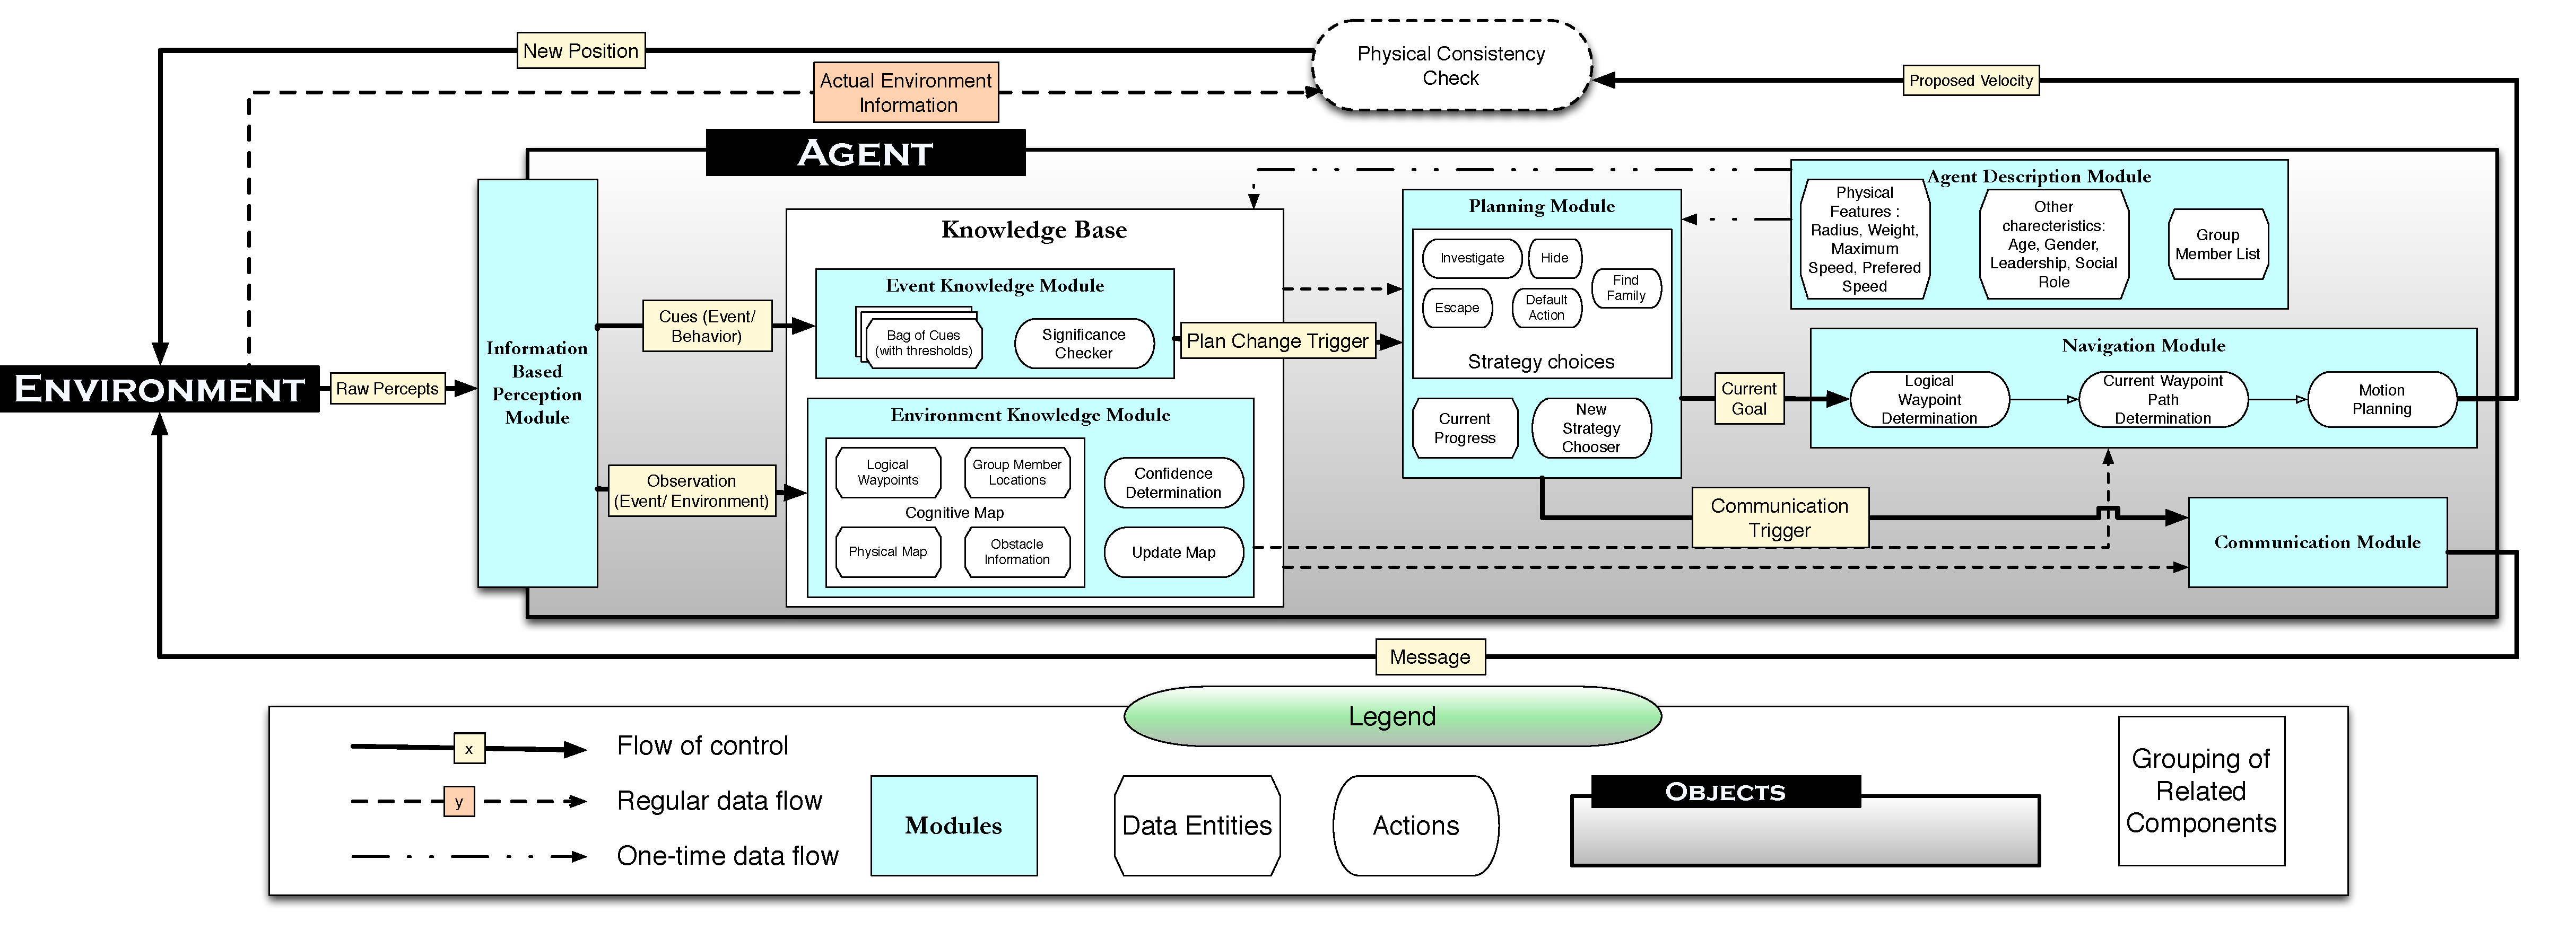
\includegraphics[width=\textwidth]{fig-AgentArchitecture}
% \caption[The Agent Architecture]{An illustrated representation of the agent architecture described in Section~\ref{IBEVAC:AgentArchitecture}}
% \label{fig:AgentArchitecture}
% \end{sidewaysfigure}

\subsection{An Information Processing Based Model of Perception}
\label{IBEVAC:IBPModule}

Traditionally, it is standard practice to model agents as having a simple circular or elliptical sensor range. All agents and objects within that sensor range are perceived by the perceiving agent. The MASSegress model~\cite{Pan:2006vp} takes a different approach of using a ray tracing algorithm. Perception models in general do not take into consideration the limitations of human information processing capacity~\cite{Miller:1956tr}. The limited information processing capacity also leads to chunking of information by the human brain. Modeling this limited information processing capacity and chunking can produce significant improvements in the realism of crowd simulations. This is demonstrated in Chapter~\ref{chapter:IBP} which introduces the Information Based Perception model which takes this into account.
% There are many objects or actions that an agent can sense or observe in the environment. We call these \emph{raw percepts}. There are many different ways according to which these raw percepts can be classified. According to the sources, they can be classified as \emph{observations} from the environment and \emph{messages} from other agents.

% Observations themselves can either be observations about the static objects in the environment or the actions of other agents in the environment~(a group of people running away from something). Regardless of the kind of message, perception is the only gateway through which the agent receives information from the environment. Given the kind of information present in the percepts, the IBP module passes this on to either the Knowledge Base or the Navigation Module. The working of module is described in detail in Chapter~\ref{chapter:IBP}.

% \subsection{Knowledge Base}
% \label{IBEVAC:KnowledgeBase}

% The Knowledge Base is responsible for storing the beliefs of the agent. It stores all the information that the agent currently has about the environment and the situation. This information or knowledge consists of two things: Event Knowledge and the Environment Knowledge.

\subsection{Modeling an event identification system}
\label{IBEVAC:EventKnowledgeModule}



% The Event Knowledge Module stores the agent's beliefs about the current state of the environment.
As discussed in Section~\ref{IBEVAC:EgressProgress}, an evacuee perceiving cues and associating them with an event and thus identifying the event is a key component of a behavior model of egress.
% In essence, there is a need for an agent to keep a track of the phase of evacuatio.
% Event identification can be considered to be equivalent to the process of associating perceived cues with an experience in a Recognition Primed D.
Chapter~\ref{chapter:PreEvacuationBehavior} introduces a model for event identification that enables the modeling of pre-evacuation behavior and studying of it's effects. Briefly, the proposed Event Knowledge Module consists of multiple \emph{buckets} of information each with a specified threshold. Each bucket signifies the belief of the agent that a particular stage in egress has been reached. The value of these thresholds are determined by the characteristics of the agents like it's social role, training, age, gender and other characteristics. An overflowing bucket triggers the planner to change its current plan. Each event or behavioral cue received is placed into one of the buckets. Once the amount of information available from the cues in the bucket crosses the threshold a trigger is sent to the planner.


\subsection{Making an evacuation plan}
\label{IBEVAC:EnvironmentKnowledgeModule}

% The \emph{Environment Knowledge Module} stores the agents personal map. This map is the representation of the layout of the environment that the agent is trying to escape that is formed as a result of the observations and experiences of the agent in the environment. The formation of environment knowledge is dependent on the exploration strategy of the evacuees and their behavior in general. However, as is discussed in Chapter~\ref{chapter:SpatialKnowledgeChapter}, existing studies on knowledge formation and the use of partial knowledge are few. Hence, this thesis introduces a game based methodology for studying this. This new methodology and the resulting model are presented in Chapter~\ref{chapter:SpatialKnowledgeChapter}.




% \subsection{Agent Description Module~(ADM)}
% \label{IBEVAC:AgentDescriptionModule}

% This module describes the agent by specifying the properties/~characteristics of the agent. This includes the features of the individual like age, gender, speed, mass and height.All these factors influence the thresholds in the Event Knowledge Module. Some of these factors are given in Table~\ref{tab:Cues}.

% \subsection{Planning Module}
% \label{IBEVAC:PlanningModule}
% The Planning Module creates a plan of action for the agent as a set of tasks. In the current scenario each \emph{task} is just a location that the agent has to go to. This goal is passed to the Navigation Module to determine how exactly to get to that location. The Planning module is shaped by the Agent Description Module, triggered by the Event Knowledge Module and informed by the Environment Knowledge Module. Generally, the planning module has \emph{strategies} for normal action, investigation, escaping and taking shelter. Each strategy, while not described completely, does give a set of tasks that the agent is supposed to complete for that strategy and this might vary according to the internals of the ADM. The tasks involved in \emph{investigation} would be to find locations of exits and to verify the existence of fire. The planner, based on the information that it has, will determine the location on the map to move to in order to get the next task done and pass this as the current goal to the Navigation Module. By controlling the state of the agent, the planning module is also indirectly responsible for determining communication. Depending on the type of agent and its state a communication trigger is sent to the communication module to communicate messages with other agents.

% The Planning Module or the Planner is responsible for determining the behavior of the agent and the actions that it undertakes at any given point of time. It receives triggers from the Event Knowledge Module that triggers a change in behavior. The new plan of action is determined by the information of the environment available from the environment knowledge module. The strategies taken are also shaped by the features of the agent described by the ADM which at the time of creation determines the strategies that are available to each agent. Beyond this the exact strategy taken by the agent at a given point of time is dependent on the information available to the agent at that point of time.

On identifying that the situation requires evacuation, an evacuee develops a plan for evacuation. Ideally, this plan would be to move towards the closest exit that is known. In most cases, however, like a shopping mall or a hospital, it is highly likely that the majority of the occupants do not know emergency exit locations or the closest exits. How evacuees explore and form their memory in such a situation of partial knowledge is still an open problem that needs to addressed. Existing simulations either assume complete knowledge or have a simplistic memory model where a single visit is remembered forever. Chapter~\ref{chapter:SpatialKnowledgeChapter} reveals how this is clearly not the case. The chapter introduces a game based methodology for studying exploration of indoor environments. By comparing against a pure random walker, it is shown that humans are in fact more effective explorers than a random walker but not as efficient as is portrayed in existing computational models of egress.

% The output of the Planner is a goal that is sent to the Navigation Module, which in turn determines the path and movement towards that point. A new goal sent to the Navigation Module initiates a recalculation of the path to be taken in the Navigation Module.
% The Planner also makes use of timer which is used to simulate the time taken by the agent to complete a task at a particular point.

% Generally, the initial task of an agent depends on the details of the agent and the environment being modeled. In an office environment, the majority of the agents will be working at their desks in the office, a few might be waiting near a water cooler or near the toilet. These are the subjective default tasks that these agents might be engaged in. When a trigger is received from the Event Knowledge Module a new task is added to the task list: information seeking. This will cause the agent to move to specific gathering points in the environment where it is likely that people meet up; or explore the environment with the aim to categorize the situation better. This movement to the gathering point or exploration is effected by sending a new goal to the Navigation Module.

% So, in essence, the Planner module is like the central decision making module of the agent. It takes triggers from the Event Knowledge Module, and the ADM and sends goals to the Navigation Module. The Navigation Module then helps the agent move to this spot in the environment.

% \subsection{Communication Module}
% \label{IBEVAC:CommunicationModule}
%  These agents can communicate with each other and transfer their knowledge of exits and hazards in the environment to others.

%  This module encodes the information passed to it from the Knowledge Base and converts it into messages that can be perceived by other agents' IBP module. It transmits this messages to agents within a communication range provided some conditions are met. This process of communication and it's effects are discussed in more detail in Chapter~\ref{chapter:PreEvacuationBehavior} and Chapter~\ref{chapter:SpatialKnowledgeChapter}.

\subsection{Navigating towards a goal}
\label{IBEVAC:NavigationModule}

The output of the planner is a goal that is sent to the Navigation system, which in turn determines the path and movement towards that point. Navigation is defined as the process or activity of accurately ascertaining one's position and planning and following a route. We use the term \emph{Navigation} to refer to the complete process of how a person moves from one point to another. From the definition, Navigation consists of 2 distinct processes: planning a route and following the route. The former is referred to as path planning and the latter is called motion planning.



At the path planning level, the module receives a goal from the Planning Module and it outputs a path that will lead it to this goal. It provides a set of way points to move through to reach this goal. These way points are determined based on the agent's personal cognitive map and the obstacles that the agent is currently perceiving. This process can be further broken down into two parts: A higher level path finder that finds abstract logical waypoints towards the goal and a lower level mechanism that translates these logical waypoints to physical locations on the map that the agent can pass through for a collision free path to it's goal. In Fig.~\ref{fig:detailedNavigationModule}, which gives a mathematical overview of the navigation process, the former is called ``Logical Waypoint Determination'' and the latter is called ``Current Waypoint Path Determination''. This is followed by the motion planning process.

Motion planning is a term borrowed from robotics which originally means detailing a task into discrete motions. In the context of crowd simulation, we use the term motion planning to refer to the task of finding a collision free velocity to get from the current point to the next waypoint in the planned path. In Fig.~\ref{fig:AgentArchitecture}, the motion planning layer ensures that the agent manages to reach its next way point without colliding with other agents. There are several different models of motion planning that have been proposed that sometimes work in very different ways. However, there is no generally accepted approach to compare the different models and determine which is the best. Chapter~\ref{chapter:MotionPlannerComparison} gives an overview of existing models of motion planning and introduces a method to quantitatively compare and evaluate existing motion planning systems.

To explain the working of the navigation module, we make use of the illustration in Fig.~\ref{fig:detailedNavigationModule}.  In this thesis, the cognitive map is implemented as a graph with the edges indicating \emph{areas} or rooms in the environment and $E_i$ refers to an $i^{th}$ edge of the graph in the agent's cognitive map.

\begin{figure}[!tb]
\centering
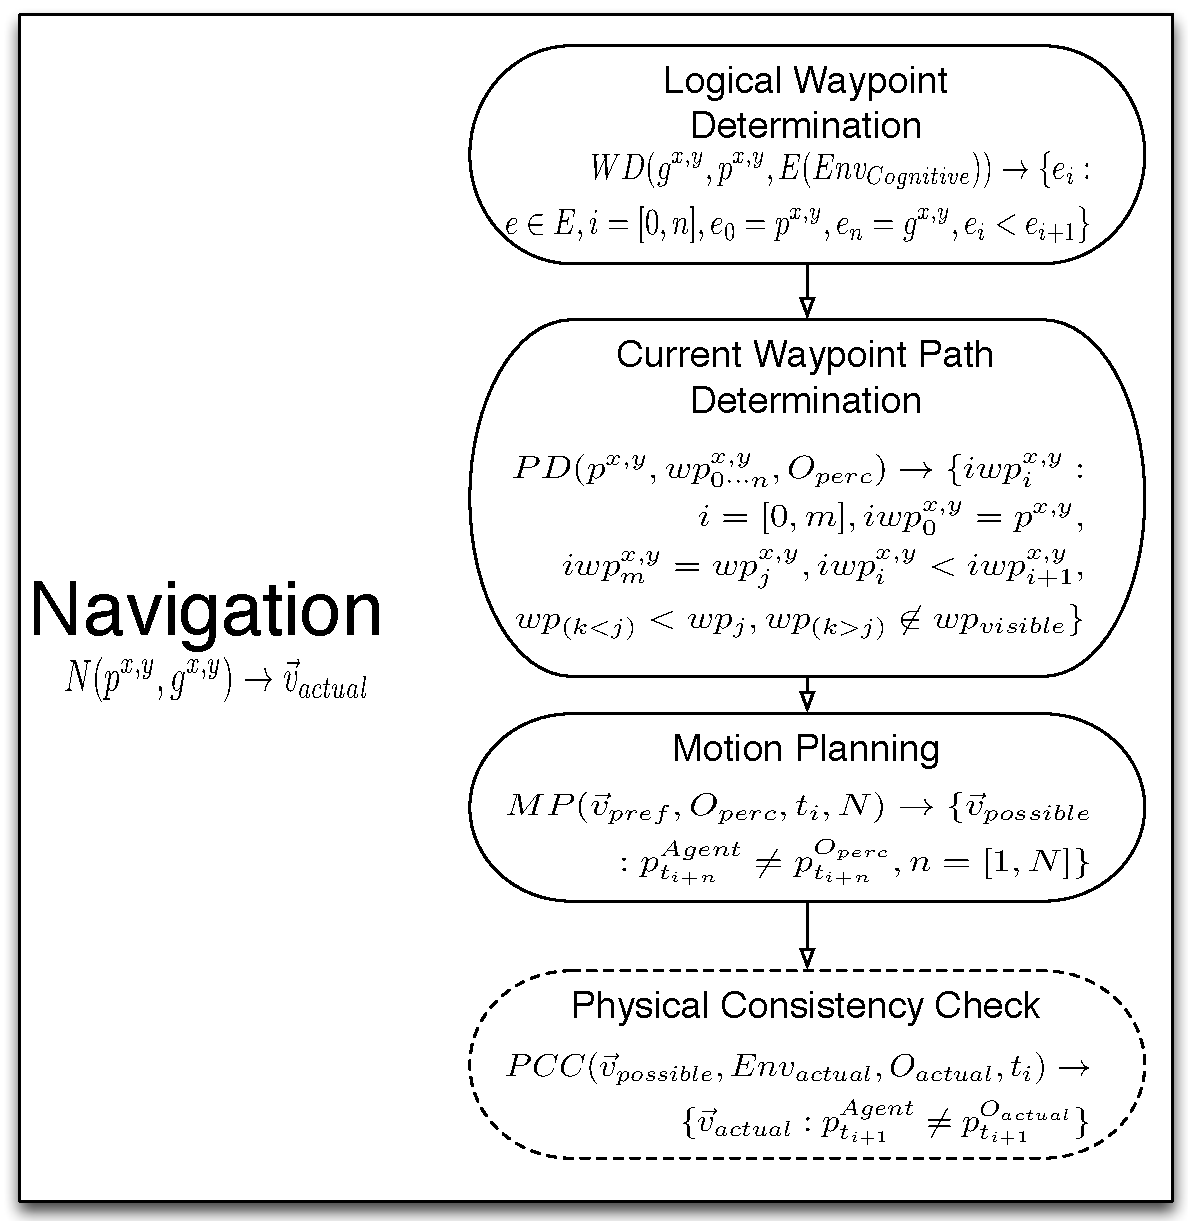
\includegraphics[height=5in]{NavigationWithFormula}
\caption[Detailed Navigation Model]{Mathematical depiction of the working of Navigation Model}
\label{fig:detailedNavigationModule}
\end{figure}

The goal position~($g^{x,y}$) is first received by the \emph{Logical Waypoint Determination}~($WD$) system which then uses a route finding algorithm like A-star or Djikstra's~\cite{Russel:1995wca} to find a set of logical waypoints~($E_i$) that will lead the agent from its current position($p^{x,y}$) to the goal position~($g^{x,y}$). The logical waypoints in the path so planned will be a list of links from the agent's cognitive map~($Env_{cognitive}$). This implies two things: Firstly, it looks at the environment at the room/ area level. Secondly, the agent plans a path according to his personal cognitive map hence there is no assurance that the path planned by two agents from the same point will be exactly the same. This step is called a waypoint determination step because it returns a set of logical waypoints to be used by the agent to reach its goal. This set of logical waypoints is then passed to the next level of navigation, i.e.\ \emph{the Current Waypoint Path Determination} step.

The \emph{Current Waypoint Path Determination}~($PD$) differs from the higher layer in that it takes into consideration dynamic obstacles i.e.\ other agents, as well as the static obstacles to determine a collision free path from the current location to the farthest visible waypoint. The logical waypoints are first converted to a set of concrete waypoints~($WP^{x,y}$) which are actual locations on the map. Using the set of perceived obstacles~($O_{perc}$) a set of intermediate waypoints~($IWP^{x,y}$) that would enable a collision free path to the farthest visible concrete waypoint~($wp^{x,y}_j$) is calculated and passed to the next level. This level can also be referred to as the \emph{strategic planning step} since it tries to model how a person strategically moves from one point to another while ensuring that it minimizes collisions with others. One possible way of doing this is by using a pattern based motion system~\cite{Nan:2011vr} or the effort minimizing algorithm ClearPath~\cite{Guy:2009gu}.

The preferred velocity of the agent is then set to velocity that would lead it to the next intermediate concrete waypoint. There are several popular collision avoidance algorithms likes Reciprocal Velocity Obstacles~\cite{Guy:2010ko,Yeh:2008tg} and Social force~\cite{Helbing:1995ie} based methods. As mentioned above, these will be discussed in more detail in Chapter~\ref{chapter:MotionPlannerComparison}. Their basic working is that at each time step~($t_i$), these algorithms take a preferred velocity~($\vec{v}_{pref}$) and set of obstacles~($O_{perc}$) (both static and dynamic) as input and output a possible velocity~($\vec{v}_{possible}$) that the agent can use to ensure that collisions do not occur for the next $N$ seconds. The two important points of difference from the previous layer is that it has some noticeable effect only when a collision is imminent and that it is very short term (limited to a few time steps) as compared to PD.

% Since the Motion Planning system works on the basis of perceived obstacles and not actual obstacles, there is a chance, especially in dense environments, that the predicted velocity might cause a collision. In such cases, the lowest level \emph{Physical Consistency Check}~($PCC$) layer ensures that unnatural behavior is not produced. As the name suggests, this layer ensures that physical consistency is maintained and people don't walk through other people and static obstacles in the environment during the next time step~($t_{i+1}$). This is the only layer in the agent that uses the actual map($Env_{actual}$) and actual obstacles($O_{actual}$) instead of the personal cognitive map and perceived obstacles.

In summary, the Navigation system receives a goal that is passed to the highest level which determines a high level route through the different areas in the environment to the goal; this waypoint is passed to the next level which determines a path towards the current waypoint that avoids dynamic obstacles and calculates the velocity of the agent to get to the waypoint while avoiding collisions for the next time step of the simulation.




% REMEMBER TO REMOVE THE PHYSICAL CONSISTENCY CHECK FROM THE AGENT ARCHITECTURE.

\section{Summary}
\label{IBEVAC:Summary}

% This chapter introduced the IBEVAC Agent Architecture for modeling complex behavior in agent based simulations of crowds. This architecture consists of and \emph{Information Based Perception Module} as a sensor, a \emph{Knowledge Base} consisting of both events and the environment, an \emph{Agent Descriptor Module} which could be used to specify the properties of the agents, a \emph{Planning Module} for planning and a \emph{Navigation Module} and \emph{Communication Module} as actuators. The rest of the thesis develops each of these components to form.

This chapter first summarized the behavior of an evacuee during evacuation from the literature in the previous Chapter. Following this, the process of evacuation was broken down into four building blocks. The final section, introduced the contributions of this paper in improving the models of each of these building blocks.